\documentclass{beamer}
\usepackage[utf8]{inputenc}
\usepackage{amsmath,amssymb}
\usepackage{mathtools}
\usepackage{bm}
\usepackage{tikz}
\usepackage{pgfplots}
\pgfplotsset{compat=1.16}

\usetheme{Madrid}
\usecolortheme{default}

\title{Bias-Variance Tradeoff in Statistical Learning}
\author{}
\date{\today}

\begin{document}

%%%%%%%%%%%%%%%%%%%%%%%%%%%%%%%%%%%%%%%%%%%%%%%%%%%%%%%%%%%%%%%
% Title Slide
%%%%%%%%%%%%%%%%%%%%%%%%%%%%%%%%%%%%%%%%%%%%%%%%%%%%%%%%%%%%%%%
\begin{frame}
  \titlepage
\end{frame}

%%%%%%%%%%%%%%%%%%%%%%%%%%%%%%%%%%%%%%%%%%%%%%%%%%%%%%%%%%%%%%%
% Frame: Outline
%%%%%%%%%%%%%%%%%%%%%%%%%%%%%%%%%%%%%%%%%%%%%%%%%%%%%%%%%%%%%%%
\begin{frame}{Outline}
  \tableofcontents
\end{frame}

%%%%%%%%%%%%%%%%%%%%%%%%%%%%%%%%%%%%%%%%%%%%%%%%%%%%%%%%%%%%%%%
% Section: Introduction
%%%%%%%%%%%%%%%%%%%%%%%%%%%%%%%%%%%%%%%%%%%%%%%%%%%%%%%%%%%%%%%
\section{Introduction to Bias and Variance}

\begin{frame}{Fundamental Concepts: Bias and Variance}
  \begin{definition}[Bias]
    The bias of an estimator $\hat{\theta}$ for a parameter $\theta$ is:
    \[
    \text{Bias}(\hat{\theta}) = \mathbb{E}[\hat{\theta}] - \theta
    \]
  \end{definition}
  
  \begin{definition}[Variance]
    The variance of an estimator $\hat{\theta}$ is:
    \[
    \text{Var}(\hat{\theta}) = \mathbb{E}[(\hat{\theta} - \mathbb{E}[\hat{\theta}])^2]
    \]
  \end{definition}
  
  \begin{block}{Interpretation}
    \begin{itemize}
      \item \textbf{Bias:} Systematic error; how far predictions are from true values on average
      \item \textbf{Variance:} Statistical dispersion; how much predictions fluctuate
    \end{itemize}
  \end{block}
\end{frame}

\begin{frame}{Target Shooting Analogy}
  \begin{columns}
    \begin{column}{0.5\textwidth}
      \begin{center}
        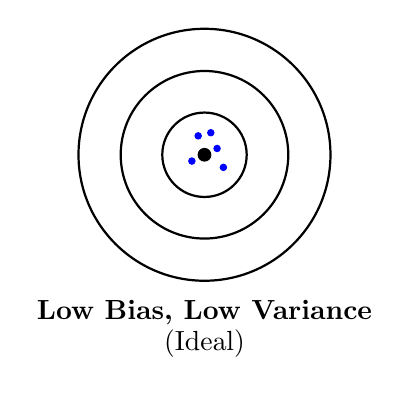
\begin{tikzpicture}[scale=0.8]
          \draw[thick] (0,0) circle (2);
          \draw[thick] (0,0) circle (1.33);
          \draw[thick] (0,0) circle (0.67);
          \filldraw[black] (0,0) circle (0.1);
          
          % Low bias, low variance (top left)
          \filldraw[blue] (0.2,0.1) circle (0.05);
          \filldraw[blue] (0.3,-0.2) circle (0.05);
          \filldraw[blue] (-0.1,0.3) circle (0.05);
          \filldraw[blue] (-0.2,-0.1) circle (0.05);
          \filldraw[blue] (0.1,0.35) circle (0.05);
          
          \node at (0,-2.5) {\textbf{Low Bias, Low Variance}};
          \node at (0,-3) {(Ideal)};
        \end{tikzpicture}
      \end{center}
    \end{column}
    
    \begin{column}{0.5\textwidth}
      \begin{center}
        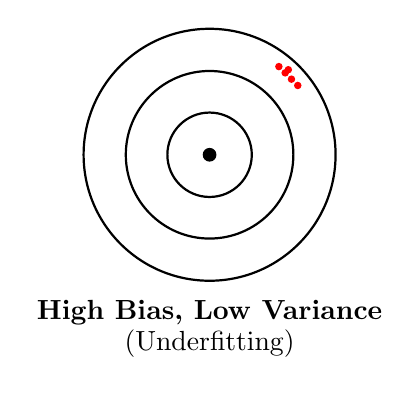
\begin{tikzpicture}[scale=0.8]
          \draw[thick] (0,0) circle (2);
          \draw[thick] (0,0) circle (1.33);
          \draw[thick] (0,0) circle (0.67);
          \filldraw[black] (0,0) circle (0.1);
          
          % High bias, low variance (top right)
          \filldraw[red] (1.2,1.3) circle (0.05);
          \filldraw[red] (1.3,1.2) circle (0.05);
          \filldraw[red] (1.1,1.4) circle (0.05);
          \filldraw[red] (1.4,1.1) circle (0.05);
          \filldraw[red] (1.25,1.35) circle (0.05);
          
          \node at (0,-2.5) {\textbf{High Bias, Low Variance}};
          \node at (0,-3) {(Underfitting)};
        \end{tikzpicture}
      \end{center}
    \end{column}
  \end{columns}
\end{frame}

\begin{frame}{Target Shooting Analogy (continued)}
  \begin{columns}
    \begin{column}{0.5\textwidth}
      \begin{center}
        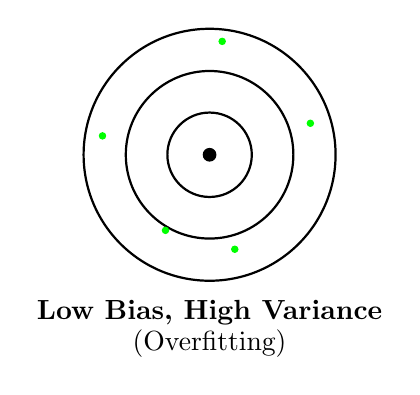
\begin{tikzpicture}[scale=0.8]
          \draw[thick] (0,0) circle (2);
          \draw[thick] (0,0) circle (1.33);
          \draw[thick] (0,0) circle (0.67);
          \filldraw[black] (0,0) circle (0.1);
          
          % Low bias, high variance (bottom left)
          \filldraw[green] (0.2,1.8) circle (0.05);
          \filldraw[green] (-1.7,0.3) circle (0.05);
          \filldraw[green] (0.4,-1.5) circle (0.05);
          \filldraw[green] (1.6,0.5) circle (0.05);
          \filldraw[green] (-0.7,-1.2) circle (0.05);
          
          \node at (0,-2.5) {\textbf{Low Bias, High Variance}};
          \node at (0,-3) {(Overfitting)};
        \end{tikzpicture}
      \end{center}
    \end{column}
    
    \begin{column}{0.5\textwidth}
      \begin{center}
        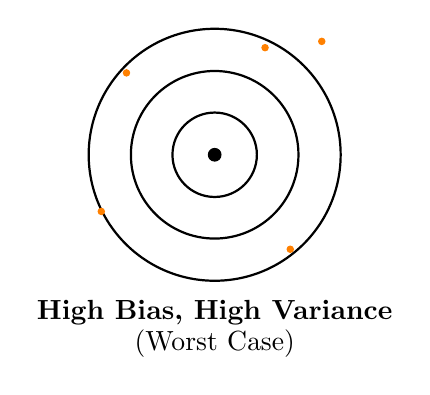
\begin{tikzpicture}[scale=0.8]
          \draw[thick] (0,0) circle (2);
          \draw[thick] (0,0) circle (1.33);
          \draw[thick] (0,0) circle (0.67);
          \filldraw[black] (0,0) circle (0.1);
          
          % High bias, high variance (bottom right)
          \filldraw[orange] (1.7,1.8) circle (0.05);
          \filldraw[orange] (1.2,-1.5) circle (0.05);
          \filldraw[orange] (-1.4,1.3) circle (0.05);
          \filldraw[orange] (-1.8,-0.9) circle (0.05);
          \filldraw[orange] (0.8,1.7) circle (0.05);
          
          \node at (0,-2.5) {\textbf{High Bias, High Variance}};
          \node at (0,-3) {(Worst Case)};
        \end{tikzpicture}
      \end{center}
    \end{column}
  \end{columns}
\end{frame}

%%%%%%%%%%%%%%%%%%%%%%%%%%%%%%%%%%%%%%%%%%%%%%%%%%%%%%%%%%%%%%%
% Section: Bias-Variance Decomposition
%%%%%%%%%%%%%%%%%%%%%%%%%%%%%%%%%%%%%%%%%%%%%%%%%%%%%%%%%%%%%%%
\section{The Bias-Variance Decomposition}

\begin{frame}{The Bias-Variance Decomposition}
  \begin{block}{Theorem}
    For a given point $x$, the expected mean squared error can be decomposed as:
    \[
    \mathbb{E}[(y - \hat{f}(x))^2] = \underbrace{(f(x) - \mathbb{E}[\hat{f}(x)])^2}_{\text{Bias}^2} + \underbrace{\mathbb{E}[(\hat{f}(x) - \mathbb{E}[\hat{f}(x)])^2]}_{\text{Variance}} + \underbrace{\sigma^2_\varepsilon}_{\text{Irreducible Error}}
    \]
  \end{block}

  \begin{itemize}
    \item $f(x)$ is the true function
    \item $\hat{f}(x)$ is our model's prediction
    \item $\sigma^2_\varepsilon$ is the noise variance (can't be reduced)
  \end{itemize}
\end{frame}

\begin{frame}{Proof Sketch of the Decomposition}
  Let $y = f(x) + \varepsilon$ where $\mathbb{E}[\varepsilon] = 0$ and $\text{Var}(\varepsilon) = \sigma^2_\varepsilon$.
  
  \begin{enumerate}
    \item Start with the expected squared error:
    \[
    \mathbb{E}[(y - \hat{f}(x))^2] = \mathbb{E}[(f(x) + \varepsilon - \hat{f}(x))^2]
    \]
    
    \item Expand and use $\mathbb{E}[\varepsilon] = 0$:
    \[
    = \mathbb{E}[(f(x) - \hat{f}(x))^2] + \sigma^2_\varepsilon
    \]
    
    \item Add and subtract $\mathbb{E}[\hat{f}(x)]$:
    \[
    = \mathbb{E}[(f(x) - \mathbb{E}[\hat{f}(x)] + \mathbb{E}[\hat{f}(x)] - \hat{f}(x))^2] + \sigma^2_\varepsilon
    \]
    
    \item Expand and use $\mathbb{E}[\mathbb{E}[\hat{f}(x)] - \hat{f}(x)] = 0$:
    \[
    = (f(x) - \mathbb{E}[\hat{f}(x)])^2 + \mathbb{E}[(\hat{f}(x) - \mathbb{E}[\hat{f}(x)])^2] + \sigma^2_\varepsilon
    \]
  \end{enumerate}
\end{frame}

\begin{frame}{The Tradeoff}
  \begin{columns}
    \begin{column}{0.6\textwidth}
      \begin{itemize}
        \item Simple models: \textbf{High bias}, \textbf{low variance}
        \item Complex models: \textbf{Low bias}, \textbf{high variance}
        \item The goal: Find optimal complexity that minimizes total error
      \end{itemize}
    \end{column}
    \begin{column}{0.4\textwidth}
      \center
      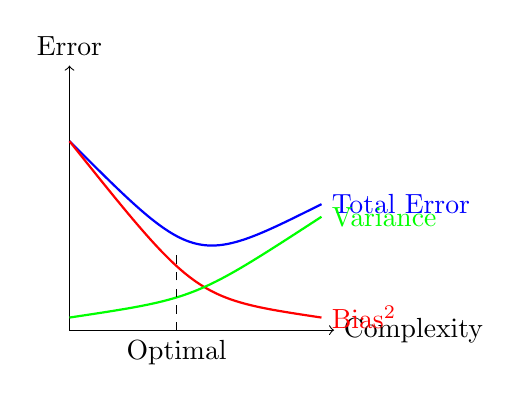
\begin{tikzpicture}[scale=0.8]
        \draw[->] (0,0) -- (4.2,0) node[right] {Complexity};
        \draw[->] (0,0) -- (0,4.2) node[above] {Error};
        \draw[thick, blue] (0,3) .. controls (2,1) .. (4,2) node[right] {Total Error};
        \draw[thick, red] (0,3) .. controls (2,0.5) .. (4,0.2) node[right] {Bias$^2$};
        \draw[thick, green] (0,0.2) .. controls (2,0.5) .. (4,1.8) node[right] {Variance};
        \draw[dashed] (1.7,0) -- (1.7,1.3);
        \node at (1.7,0) [below] {Optimal};
      \end{tikzpicture}
    \end{column}
  \end{columns}
\end{frame}

%%%%%%%%%%%%%%%%%%%%%%%%%%%%%%%%%%%%%%%%%%%%%%%%%%%%%%%%%%%%%%%
% Section: Estimator Examples
%%%%%%%%%%%%%%%%%%%%%%%%%%%%%%%%%%%%%%%%%%%%%%%%%%%%%%%%%%%%%%%
\section{Practical Examples}

\begin{frame}{Sample Mean Estimator}
  \begin{block}{Properties}
    For i.i.d. random variables $X_1, X_2, \ldots, X_n$ with mean $\mu$ and variance $\sigma^2$, the sample mean $\bar{X}_n = \frac{1}{n} \sum_{i=1}^n X_i$ has:
    \begin{align*}
    \text{Bias}(\bar{X}_n) &= \mathbb{E}[\bar{X}_n] - \mu = 0 \\
    \text{Var}(\bar{X}_n) &= \frac{\sigma^2}{n}
    \end{align*}
  \end{block}
  
  \begin{block}{Key Insights}
    \begin{itemize}
      \item The sample mean is unbiased
      \item Its variance decreases with sample size ($1/n$ rate)
      \item Larger samples provide more precise estimates
    \end{itemize}
  \end{block}
\end{frame}

\begin{frame}{Variance Estimators}
  Two common estimators for the population variance:
  
  \begin{block}{Biased (Maximum Likelihood) Estimator}
    \[
    \hat{\sigma}^2_{\text{biased}} = \frac{1}{n} \sum_{i=1}^n (X_i - \bar{X})^2
    \]
    
    Properties: $\mathbb{E}[\hat{\sigma}^2_{\text{biased}}] = \frac{n-1}{n} \sigma^2$ (underestimates true variance)
  \end{block}
  
  \begin{block}{Unbiased Estimator}
    \[
    \hat{\sigma}^2_{\text{unbiased}} = \frac{1}{n-1} \sum_{i=1}^n (X_i - \bar{X})^2
    \]
    
    Properties: $\mathbb{E}[\hat{\sigma}^2_{\text{unbiased}}] = \sigma^2$ (no bias)
  \end{block}
  
  Despite being biased, the MLE might have lower MSE for small samples (bias-variance tradeoff)
\end{frame}

%%%%%%%%%%%%%%%%%%%%%%%%%%%%%%%%%%%%%%%%%%%%%%%%%%%%%%%%%%%%%%%
% Section: Shrinkage Estimators
%%%%%%%%%%%%%%%%%%%%%%%%%%%%%%%%%%%%%%%%%%%%%%%%%%%%%%%%%%%%%%%
\section{Shrinkage Estimators}

\begin{frame}{Introduction to Shrinkage}
  \begin{block}{Concept}
    Shrinkage estimators deliberately introduce bias to reduce variance, potentially achieving lower overall error
  \end{block}
  
  \begin{itemize}
    \item "Shrink" estimates toward a target value
    \item Trade off increased bias for reduced variance
    \item Can outperform unbiased estimators in terms of MSE
  \end{itemize}
  
  \begin{block}{General Form}
    \[
    \hat{\theta}_{\alpha} = (1-\alpha) \hat{\theta}_{\text{unbiased}} + \alpha \, \theta_{\text{target}}
    \]
    where $\alpha \in [0,1]$ is the shrinkage parameter
  \end{block}
\end{frame}

\begin{frame}{Properties of Shrinkage Estimators}
  For the shrinkage estimator $\hat{\theta}_{\alpha} = (1-\alpha) \hat{\theta}_{\text{unbiased}} + \alpha \, \theta_{\text{target}}$:
  
  \begin{block}{Bias and Variance}
    \begin{align*}
    \text{Bias}(\hat{\theta}_{\alpha}) &= \alpha(\theta_{\text{target}} - \theta) \\
    \text{Var}(\hat{\theta}_{\alpha}) &= (1-\alpha)^2 \text{Var}(\hat{\theta}_{\text{unbiased}})
    \end{align*}
  \end{block}
  
  \begin{block}{Mean Squared Error}
    \begin{align*}
    \text{MSE}(\hat{\theta}_{\alpha}) &= \text{Bias}(\hat{\theta}_{\alpha})^2 + \text{Var}(\hat{\theta}_{\alpha}) \\
    &= \alpha^2(\theta_{\text{target}} - \theta)^2 + (1-\alpha)^2 \text{Var}(\hat{\theta}_{\text{unbiased}})
    \end{align*}
  \end{block}
\end{frame}

\begin{frame}{Optimal Shrinkage Parameter}
  \begin{block}{Derivation}
    To find the optimal $\alpha^*$, differentiate MSE with respect to $\alpha$ and set to zero:
    
    \begin{align*}
    \frac{d}{d\alpha} \text{MSE}(\hat{\theta}_{\alpha}) &= 2\alpha(\theta_{\text{target}} - \theta)^2 - 2(1-\alpha) \text{Var}(\hat{\theta}_{\text{unbiased}}) = 0
    \end{align*}
    
    Solving for $\alpha$:
    \begin{align*}
    \alpha^* &= \frac{\text{Var}(\hat{\theta}_{\text{unbiased}})}{(\theta_{\text{target}} - \theta)^2 + \text{Var}(\hat{\theta}_{\text{unbiased}})}
    \end{align*}
  \end{block}
  
  \begin{block}{Insights}
    \begin{itemize}
      \item Stronger shrinkage when variance is high
      \item Stronger shrinkage when target is close to true value
      \item Optimal $\alpha^*$ depends on unknown parameters (need estimation in practice)
    \end{itemize}
  \end{block}
\end{frame}

\begin{frame}{Example: James-Stein Estimator}
  \begin{block}{Setting}
    Estimating means $\boldsymbol{\mu} = (\mu_1, \ldots, \mu_p)^T$ of a multivariate normal with $p \geq 3$ components
  \end{block}
  
  \begin{block}{James-Stein Estimator}
    \[
    \hat{\boldsymbol{\mu}}^{JS} = \left(1 - \frac{(p-2)\sigma^2}{\|\bar{\mathbf{X}}\|^2}\right) \bar{\mathbf{X}}
    \]
  \end{block}
  
  \begin{block}{"Paradox"}
    The James-Stein estimator has lower expected squared error than the MLE (sample mean) for \textit{any} true value of $\boldsymbol{\mu}$, despite introducing bias
  \end{block}
  
  This example shows that unbiased estimators are not always optimal in terms of MSE
\end{frame}

%%%%%%%%%%%%%%%%%%%%%%%%%%%%%%%%%%%%%%%%%%%%%%%%%%%%%%%%%%%%%%%
% Section: Model Complexity and Regularization
%%%%%%%%%%%%%%%%%%%%%%%%%%%%%%%%%%%%%%%%%%%%%%%%%%%%%%%%%%%%%%%
\section{Model Complexity and Regularization}

\begin{frame}{Underfitting vs. Overfitting}
  \begin{itemize}
    \item \textbf{Underfitting:} Model is too simple (high bias, low variance)
    \begin{itemize}
      \item Misses important patterns in the data
      \item Performs poorly on both training and test data
    \end{itemize}
    
    \item \textbf{Overfitting:} Model is too complex (low bias, high variance)
    \begin{itemize}
      \item Captures noise in the training data
      \item Performs well on training data but poorly on test data
    \end{itemize}
    
    \item \textbf{Good fit:} Appropriate complexity (balanced bias and variance)
    \begin{itemize}
      \item Captures main patterns without fitting noise
      \item Generalizes well to new data
    \end{itemize}
  \end{itemize}
\end{frame}

\begin{frame}{Polynomial Regression Example}
  Consider modeling data with polynomials of different degrees:
  
  \begin{columns}
    \begin{column}{0.33\textwidth}
      \begin{center}
        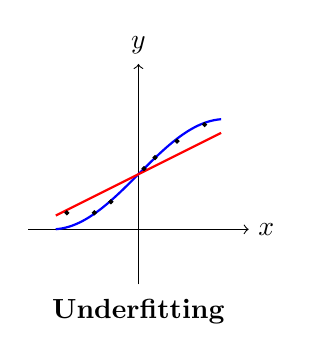
\begin{tikzpicture}[scale=0.7]
          \draw[->] (-2,0) -- (2,0) node[right] {$x$};
          \draw[->] (0,-1) -- (0,3) node[above] {$y$};
          
          % True function
          \draw[domain=-1.5:1.5, samples=50, smooth, thick, blue] 
            plot (\x, {1 + sin(deg(\x))});
          
          % Linear model (underfitting)
          \draw[domain=-1.5:1.5, samples=2, red, thick] 
            plot (\x, {1 + 0.5*\x});
          
          % Data points
          \filldraw (0.3,1.3) circle (1pt);
          \filldraw (-0.8,0.3) circle (1pt);
          \filldraw (0.1,1.1) circle (1pt);
          \filldraw (-0.5,0.5) circle (1pt);
          \filldraw (1.2,1.9) circle (1pt);
          \filldraw (0.7,1.6) circle (1pt);
          \filldraw (-1.3,0.3) circle (1pt);
          
          \node at (0,-1.5) {\textbf{Underfitting}};
        \end{tikzpicture}
      \end{center}
    \end{column}
    
    \begin{column}{0.33\textwidth}
      \begin{center}
        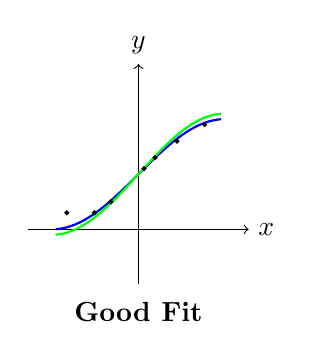
\begin{tikzpicture}[scale=0.7]
          \draw[->] (-2,0) -- (2,0) node[right] {$x$};
          \draw[->] (0,-1) -- (0,3) node[above] {$y$};
          
          % True function
          \draw[domain=-1.5:1.5, samples=50, smooth, thick, blue] 
            plot (\x, {1 + sin(deg(\x))});
          
          % Cubic model (good fit)
          \draw[domain=-1.5:1.5, samples=50, smooth, green, thick] 
            plot (\x, {1 + 1.1*sin(deg(\x))});
          
          % Data points
          \filldraw (0.3,1.3) circle (1pt);
          \filldraw (-0.8,0.3) circle (1pt);
          \filldraw (0.1,1.1) circle (1pt);
          \filldraw (-0.5,0.5) circle (1pt);
          \filldraw (1.2,1.9) circle (1pt);
          \filldraw (0.7,1.6) circle (1pt);
          \filldraw (-1.3,0.3) circle (1pt);
          
          \node at (0,-1.5) {\textbf{Good Fit}};
        \end{tikzpicture}
      \end{center}
    \end{column}
    
    \begin{column}{0.33\textwidth}
      \begin{center}
        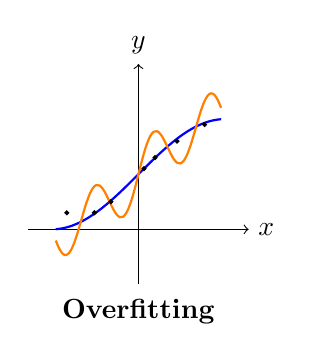
\begin{tikzpicture}[scale=0.7]
          \draw[->] (-2,0) -- (2,0) node[right] {$x$};
          \draw[->] (0,-1) -- (0,3) node[above] {$y$};
          
          % True function
          \draw[domain=-1.5:1.5, samples=50, smooth, thick, blue] 
            plot (\x, {1 + sin(deg(\x))});
          
          % High-degree polynomial (overfitting)
          \draw[domain=-1.5:1.5, samples=50, smooth, orange, thick] 
            plot (\x, {1 + sin(deg(\x)) + 0.5*sin(6*deg(\x))});
          
          % Data points
          \filldraw (0.3,1.3) circle (1pt);
          \filldraw (-0.8,0.3) circle (1pt);
          \filldraw (0.1,1.1) circle (1pt);
          \filldraw (-0.5,0.5) circle (1pt);
          \filldraw (1.2,1.9) circle (1pt);
          \filldraw (0.7,1.6) circle (1pt);
          \filldraw (-1.3,0.3) circle (1pt);
          
          \node at (0,-1.5) {\textbf{Overfitting}};
        \end{tikzpicture}
      \end{center}
    \end{column}
  \end{columns}
\end{frame}

\begin{frame}{Regularization Techniques}
  \begin{block}{Ridge Regression (L2 regularization)}
    \[
    \min_{\boldsymbol{\beta}} \|y - X\boldsymbol{\beta}\|^2 + \lambda \|\boldsymbol{\beta}\|^2
    \]
    \begin{itemize}
      \item Shrinks all coefficients toward zero
      \item Solution: $\hat{\boldsymbol{\beta}}^{\text{ridge}} = (X^TX + \lambda I)^{-1}X^Ty$
    \end{itemize}
  \end{block}
  
  \begin{block}{Lasso Regression (L1 regularization)}
    \[
    \min_{\boldsymbol{\beta}} \|y - X\boldsymbol{\beta}\|^2 + \lambda \|\boldsymbol{\beta}\|_1
    \]
    \begin{itemize}
      \item Can set some coefficients exactly to zero (feature selection)
      \item No closed-form solution
    \end{itemize}
  \end{block}
  
  \begin{block}{Elastic Net}
    \[
    \min_{\boldsymbol{\beta}} \|y - X\boldsymbol{\beta}\|^2 + \lambda_1 \|\boldsymbol{\beta}\|_1 + \lambda_2 \|\boldsymbol{\beta}\|^2
    \]
    \begin{itemize}
      \item Combines advantages of Ridge and Lasso
    \end{itemize}
  \end{block}
\end{frame}

%%%%%%%%%%%%%%%%%%%%%%%%%%%%%%%%%%%%%%%%%%%%%%%%%%%%%%%%%%%%%%%
% Section: Practical Implications
%%%%%%%%%%%%%%%%%%%%%%%%%%%%%%%%%%%%%%%%%%%%%%%%%%%%%%%%%%%%%%%
\section{Practical Implications}

\begin{frame}{Sample Size Considerations}
  \begin{itemize}
    \item \textbf{Small datasets:}
    \begin{itemize}
      \item Higher risk of overfitting
      \item Use simpler models (higher bias, lower variance)
      \item Apply stronger regularization
      \item Consider data augmentation
    \end{itemize}
    
    \item \textbf{Large datasets:}
    \begin{itemize}
      \item Can use more complex models (lower bias, manageable variance)
      \item Less need for regularization
      \item More capacity to learn intricate patterns
    \end{itemize}
    
    \item \textbf{Rule of thumb:} Model complexity should increase with sample size
  \end{itemize}
\end{frame}

\begin{frame}{Ensemble Methods}
  \begin{block}{Bagging (Bootstrap Aggregating)}
    \begin{itemize}
      \item Train multiple high-variance, low-bias models on bootstrap samples
      \item Average predictions to reduce variance
      \item Example: Random Forests
    \end{itemize}
  \end{block}
  
  \begin{block}{Boosting}
    \begin{itemize}
      \item Train sequence of weak models (high bias, low variance)
      \item Each model focuses on errors of previous models
      \item Reduces bias while controlling variance
      \item Examples: AdaBoost, Gradient Boosting
    \end{itemize}
  \end{block}
  
  \begin{block}{Stacking}
    \begin{itemize}
      \item Combine predictions from different types of models
      \item Meta-learner optimizes the combination
    \end{itemize}
  \end{block}
\end{frame}

\begin{frame}{Cross-Validation for Model Selection}
  \begin{columns}
    \begin{column}{0.6\textwidth}
      \begin{enumerate}
        \item Split data into $k$ folds
        \item For each model complexity:
        \begin{itemize}
          \item Train on $k-1$ folds
          \item Evaluate on remaining fold
          \item Repeat for all folds
          \item Average results
        \end{itemize}
        \item Choose model with best validation performance
      \end{enumerate}
    \end{column}
    
    \begin{column}{0.4\textwidth}
      \begin{center}
        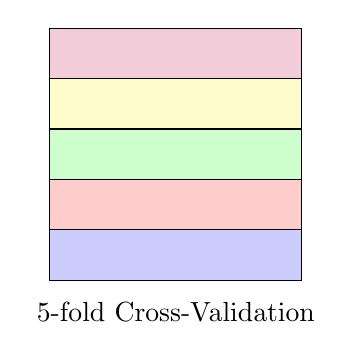
\begin{tikzpicture}[scale=0.8]
          \draw[fill=blue!20] (0,0) rectangle (4,0.8);
          \draw[fill=red!20] (0,0.8) rectangle (4,1.6);
          \draw[fill=green!20] (0,1.6) rectangle (4,2.4);
          \draw[fill=yellow!20] (0,2.4) rectangle (4,3.2);
          \draw[fill=purple!20] (0,3.2) rectangle (4,4.0);
          
          % Grid lines
          \draw (0,0.8) -- (4,0.8);
          \draw (0,1.6) -- (4,1.6);
          \draw (0,2.4) -- (4,2.4);
          \draw (0,3.2) -- (4,3.2);
          
          \node at (2,-0.5) {5-fold Cross-Validation};
        \end{tikzpicture}
      \end{center}
    \end{column}
  \end{columns}
  
  \begin{block}{Benefits}
    \begin{itemize}
      \item More reliable estimate of model performance
      \item Helps find optimal complexity without using separate test set
      \item Common choices: $k=5$ or $k=10$
    \end{itemize}
  \end{block}
\end{frame}

\begin{frame}{Experimental Results}
  \begin{center}
    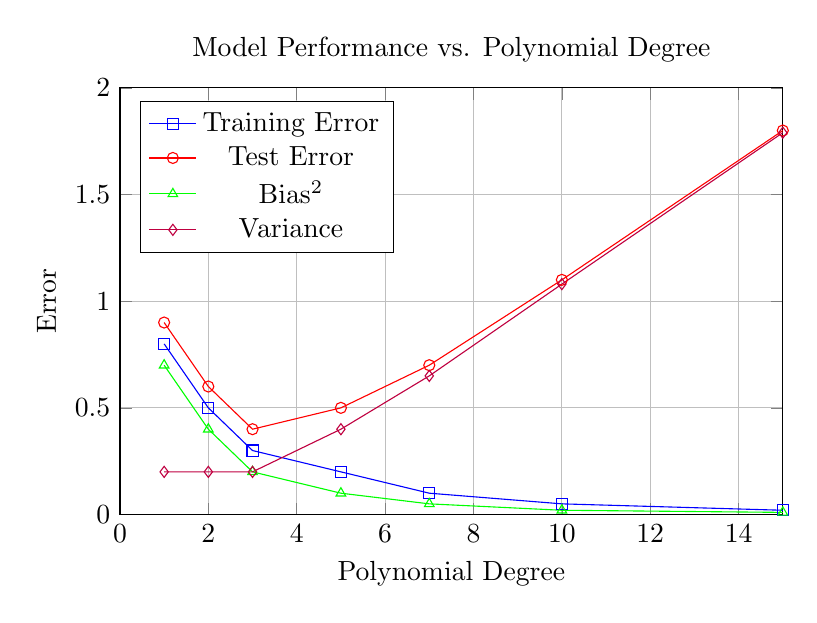
\begin{tikzpicture}
    \begin{axis}[
        title={Model Performance vs. Polynomial Degree},
        xlabel={Polynomial Degree},
        ylabel={Error},
        xmin=0, xmax=15,
        ymin=0, ymax=2,
        legend pos=north west,
        grid=major,
        width=10cm,
        height=7cm
    ]
    
    \addplot[color=blue, mark=square] coordinates {
        (1, 0.8) (2, 0.5) (3, 0.3) (5, 0.2) (7, 0.1) (10, 0.05) (15, 0.02)
    };
    \addlegendentry{Training Error};
    
    \addplot[color=red, mark=o] coordinates {
        (1, 0.9) (2, 0.6) (3, 0.4) (5, 0.5) (7, 0.7) (10, 1.1) (15, 1.8)
    };
    \addlegendentry{Test Error};
    
    \addplot[color=green, mark=triangle] coordinates {
        (1, 0.7) (2, 0.4) (3, 0.2) (5, 0.1) (7, 0.05) (10, 0.02) (15, 0.01)
    };
    \addlegendentry{Bias$^2$};
    
    \addplot[color=purple, mark=diamond] coordinates {
        (1, 0.2) (2, 0.2) (3, 0.2) (5, 0.4) (7, 0.65) (10, 1.08) (15, 1.79)
    };
    \addlegendentry{Variance};
    
    \end{axis}
    \end{tikzpicture}
  \end{center}
  
  \begin{itemize}
    \item Training error consistently decreases with model complexity
    \item Test error follows a U-shaped curve
    \item Optimal complexity balances bias and variance
  \end{itemize}
\end{frame}

%%%%%%%%%%%%%%%%%%%%%%%%%%%%%%%%%%%%%%%%%%%%%%%%%%%%%%%%%%%%%%%
% Section: Case Studies
%%%%%%%%%%%%%%%%%%%%%%%%%%%%%%%%%%%%%%%%%%%%%%%%%%%%%%%%%%%%%%%
\section{Case Studies and Applications}

\begin{frame}{Neural Network Depth and Width}
  \begin{columns}
    \begin{column}{0.6\textwidth}
      \begin{itemize}
        \item \textbf{Network depth:} Number of layers
        \begin{itemize}
          \item Deeper networks can represent more complex functions (lower bias)
          \item But harder to train and more prone to overfitting (higher variance)
        \end{itemize}
        
        \item \textbf{Network width:} Neurons per layer
        \begin{itemize}
          \item Wider networks have more parameters (lower bias)
          \item But potentially higher variance
        \end{itemize}
        
        \item \textbf{Regularization techniques:}
        \begin{itemize}
          \item Dropout: randomly deactivate neurons
          \item Weight decay: penalize large weights
          \item Early stopping: stop training before overfitting
        \end{itemize}
      \end{itemize}
    \end{column}
    
    \begin{column}{0.4\textwidth}
      \begin{center}
        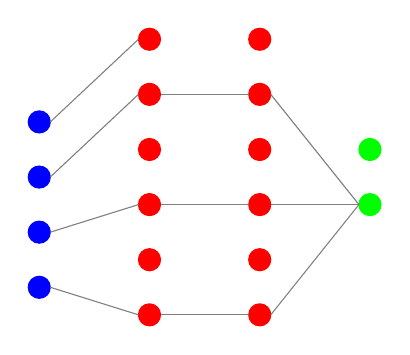
\begin{tikzpicture}[scale=0.7]
          % Input layer
          \foreach \i in {1,...,4} {
            \filldraw[blue] (0,\i) circle (0.2);
          }
          
          % First hidden layer
          \foreach \i in {1,...,6} {
            \filldraw[red] (2,\i-0.5) circle (0.2);
          }
          
          % Second hidden layer
          \foreach \i in {1,...,6} {
            \filldraw[red] (4,\i-0.5) circle (0.2);
          }
          
          % Output layer
          \foreach \i in {1,...,2} {
            \filldraw[green] (6,\i+1.5) circle (0.2);
          }
          
          % Connections (simplified)
          \draw[gray] (0.2,1) -- (1.8,0.5);
          \draw[gray] (0.2,2) -- (1.8,2.5);
          \draw[gray] (0.2,3) -- (1.8,4.5);
          \draw[gray] (0.2,4) -- (1.8,5.5);
          
          \draw[gray] (2.2,0.5) -- (3.8,0.5);
          \draw[gray] (2.2,2.5) -- (3.8,2.5);
          \draw[gray] (2.2,4.5) -- (3.8,4.5);
          
          \draw[gray] (4.2,0.5) -- (5.8,2.5);
          \draw[gray] (4.2,2.5) -- (5.8,2.5);
          \draw[gray] (4.2,4.5) -- (5.8,2.5);
        \end{tikzpicture}
      \end{center}
    \end{column}
  \end{columns}
\end{frame}

\begin{frame}{Practical Guidelines}
  \begin{enumerate}
    \item \textbf{Start simple and gradually increase complexity}
    \begin{itemize}
      \item Begin with a baseline model
      \item Incrementally increase complexity while monitoring validation performance
    \end{itemize}
    
    \item \textbf{Use cross-validation to tune model complexity}
    \begin{itemize}
      \item Find the sweet spot in the bias-variance tradeoff
    \end{itemize}
    
    \item \textbf{Consider regularization to control variance}
    \begin{itemize}
      \item L1/L2 regularization, dropout, early stopping
    \end{itemize}
    
    \item \textbf{Adjust approach based on dataset size}
    \begin{itemize}
      \item Small data: prioritize variance reduction
      \item Large data: focus on bias reduction
    \end{itemize}
    
    \item \textbf{Use ensemble methods when appropriate}
    \begin{itemize}
      \item Bagging for high-variance models
      \item Boosting for high-bias models
    \end{itemize}
  \end{enumerate}
\end{frame}

%%%%%%%%%%%%%%%%%%%%%%%%%%%%%%%%%%%%%%%%%%%%%%%%%%%%%%%%%%%%%%%
% Section: Conclusion
%%%%%%%%%%%%%%%%%%%%%%%%%%%%%%%%%%%%%%%%%%%%%%%%%%%%%%%%%%%%%%%
\section{Conclusion}

\begin{frame}{Key Takeaways}
  \begin{itemize}
    \item The bias-variance tradeoff is fundamental to understanding model performance
    \item Total error = Bias$^2$ + Variance + Irreducible Error
    \item Simple models: high bias, low variance
    \item Complex models: low bias, high variance
    \item Optimal model complexity balances bias and variance
    \item Regularization provides a way to control the tradeoff
    \item Shrinkage estimators can outperform unbiased ones
    \item Sample size affects the optimal complexity
    \item Cross-validation helps find the sweet spot
    \item Ensemble methods optimize the tradeoff
  \end{itemize}
\end{frame}

\begin{frame}{Further Reading}
  \begin{itemize}
    \item Hastie, T., Tibshirani, R., \& Friedman, J. (2009). \textit{The Elements of Statistical Learning}. Springer.
    \item James, G., Witten, D., Hastie, T., \& Tibshirani, R. (2013). \textit{An Introduction to Statistical Learning}. Springer.
    \item Bishop, C. M. (2006). \textit{Pattern Recognition and Machine Learning}. Springer.
    \item Geman, S., Bienenstock, E., \& Doursat, R. (1992). Neural Networks and the Bias/Variance Dilemma. \textit{Neural Computation}, 4(1), 1-58.
    \item Belkin, M., Hsu, D., Ma, S., \& Mandal, S. (2019). Reconciling Modern Machine-Learning Practice and the Classical Bias-Variance Trade-Off. \textit{Proceedings of the National Academy of Sciences}, 116(32), 15849-15854.
  \end{itemize}
\end{frame}

\end{document}